\subsection{Data Collection and Sources}
\label{sec:data_collection}

Our dataset comprises 649 blockchain security incident entries collected from multiple sources spanning 2016--early 2025. We employed a systematic approach to ensure comprehensive coverage while maintaining data quality and verifiability.

\begin{figure}[H]
    \centering
    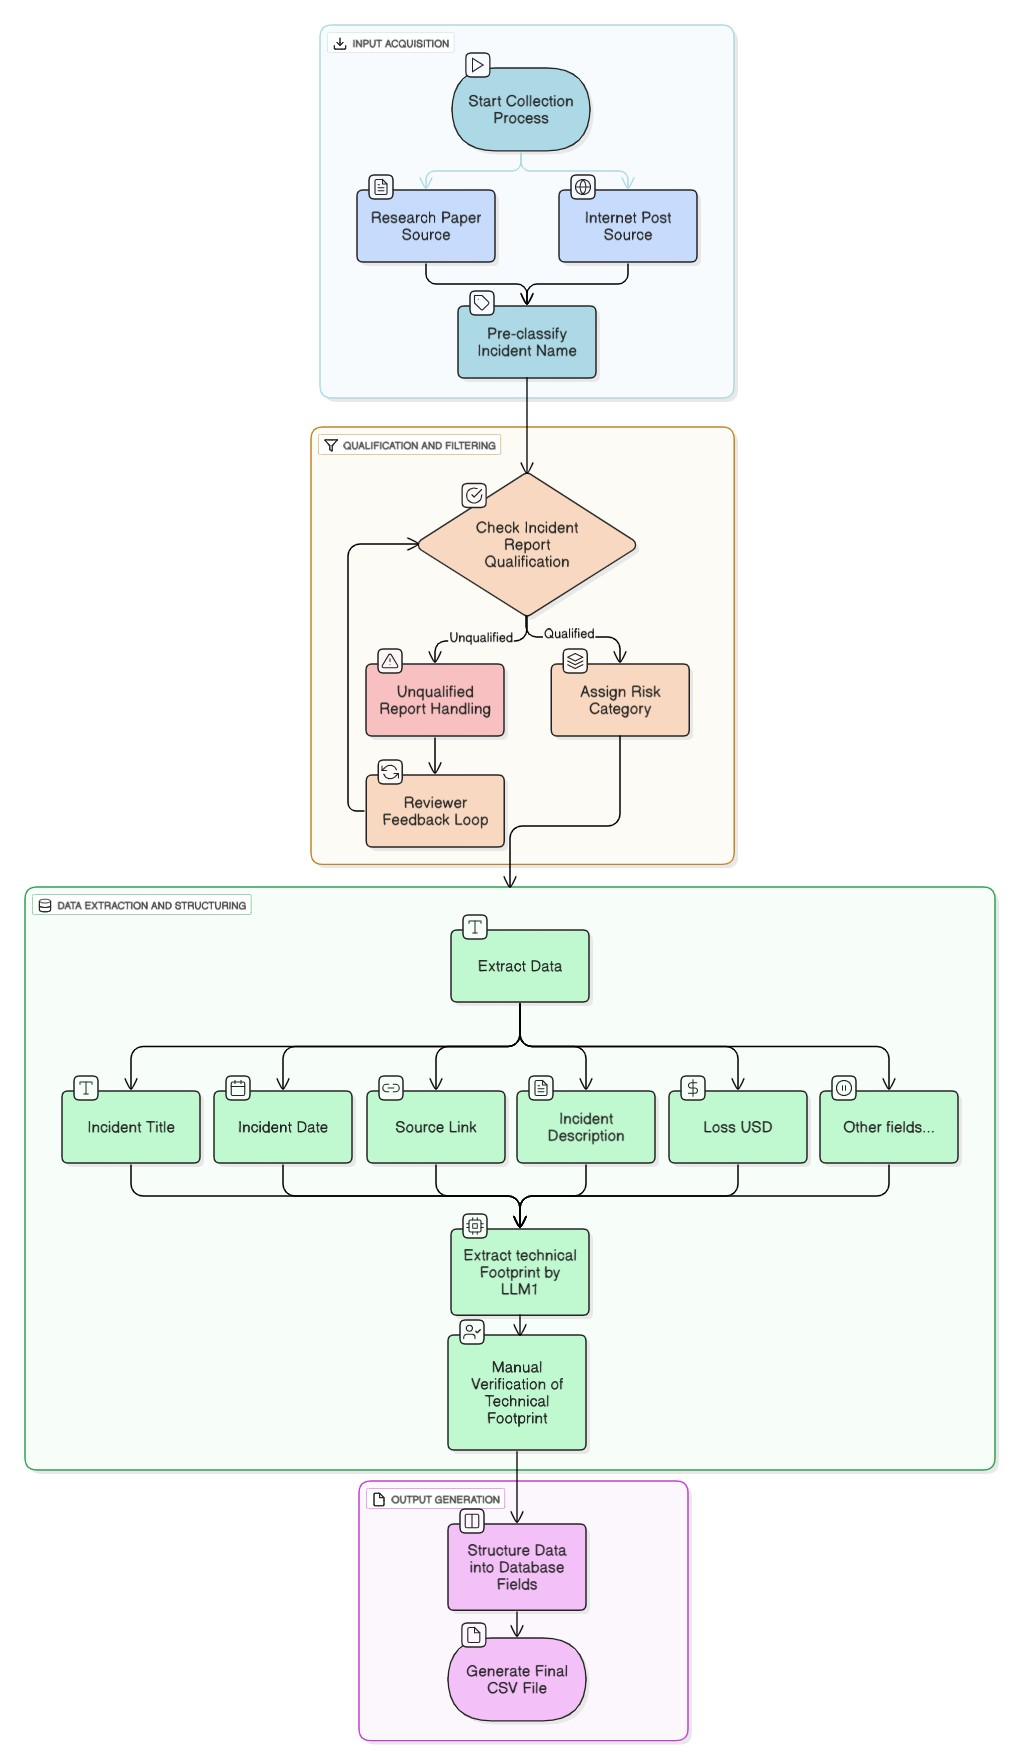
\includegraphics[width=0.4\textwidth]{../figure/methodology/collect_data.jpg}
    \caption{The process of collecting and reviewing data.}
    \label{fig:collect_data}
\end{figure}

\subsubsection{Primary Data Sources}
We collected incident data from the following primary sources:
\begin{itemize}
    \item \textbf{Web3IsGoingGreat:} A comprehensive database of blockchain security incidents with detailed incident reports and loss estimates
    \item \textbf{Rekt News:} Specialized platform tracking DeFi exploits and protocol vulnerabilities
    \item \textbf{Secureum:} Academic and industry reports on smart contract vulnerabilities and attacks
    \item \textbf{Chainalysis:} Blockchain analytics data for incident verification and impact assessment
    \item \textbf{Academic Literature:} Peer-reviewed papers and technical reports from security conferences
\end{itemize}

\subsubsection{Inclusion and Exclusion Criteria}
To ensure data quality and relevance, we applied the following criteria:

\textbf{Inclusion Criteria:}
\begin{itemize}
    \item Minimum financial loss of \$10,000 USD (adjusted for inflation)
    \item Verifiable incident reports with multiple independent sources
    \item Clear attribution to specific blockchain platforms or protocols
    \item Sufficient technical details to classify the attack vector
\end{itemize}

\textbf{Exclusion Criteria:}
\begin{itemize}
    \item Purely anecdotal or unverified reports
    \item Incidents with insufficient technical details for classification
    \item Non-blockchain related security incidents
    \item Duplicate reports of the same incident
\end{itemize}

% \begin{figure}[H]
%     \centering
%     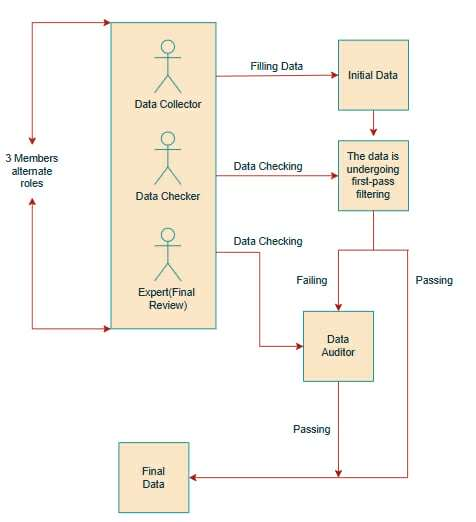
\includegraphics[width=0.3\textwidth]{../figure/methodology/peer_review.jpg}
%     \caption{Peer-reviewing data.}
%     \label{fig:peer_review}
% \end{figure} 

\subsubsection{Data Collection Protocol}
Our data collection process followed a standardized protocol:
\begin{enumerate}
    \item \textbf{Source Identification:} Systematic review of primary and secondary sources
    \item \textbf{Initial Screening:} Application of inclusion/exclusion criteria
    \item \textbf{Data Extraction:} Structured extraction of incident details, financial impact, and technical characteristics
    \item \textbf{Verification:} Cross-referencing with multiple sources for accuracy
    \item \textbf{Quality Control:} Review by multiple team members for consistency
\end{enumerate}

\subsubsection{Dataset Schema and Dictionary}

The curated incident dataset contains 649 entries structured with 18 columns. Each row corresponds to a single classified incident with complete B-SAFE framework annotations:

\begin{itemize}
    \begin{figure}[H]
        \centering
        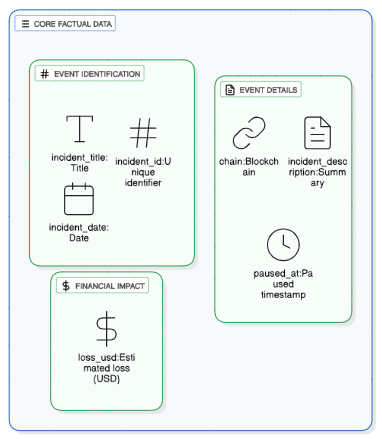
\includegraphics[width=0.3\textwidth]{../figure/methodology/core_factual_data.jpg}
        \caption{Core factual data of the dataset.}
        \label{fig:core_factual_data}
    \end{figure}
    \item \textbf{incident\_id}: Unique integer identifier for the security event
    \item \textbf{incident\_title}: Concise, descriptive title for the incident
    \item \textbf{incident\_date}: Date when the incident occurred or was first reported (MM/DD/YYYY format)
    \item \textbf{paused\_at}: Timestamp when a protocol was paused, if applicable
    \item \textbf{incident\_description}: Detailed text summary of the incident
    \item \textbf{loss\_usd}: Estimated financial loss in USD at the time of the incident
    \item \textbf{chain}: Primary blockchain or ecosystem affected (e.g., Ethereum, BNB Chain)
    \begin{figure}[H]
        \centering
        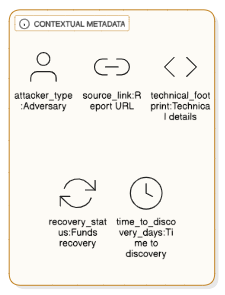
\includegraphics[width=0.3\textwidth]{../figure/methodology/contextual_metadata.jpg}
        \caption{Contextual metadata of the dataset.}
        \label{fig:contextual_data}
    \end{figure}
    \item \textbf{source\_link}: URL to a primary report or analysis of the incident
    \item \textbf{technical\_footprint}: JSON object containing structured technical details of the affected protocol, used for feature engineering
    \item \textbf{attacker\_type}: Classification of the adversary (e.g., Insider, External)
    \item \textbf{recovery\_status}: Status of the lost funds (e.g., Funds Lost, Funds Recovered)
    \item \textbf{time\_to\_discovery\_days}: Estimated time in days from exploit to public discovery
    \begin{figure}[H]
        \centering
        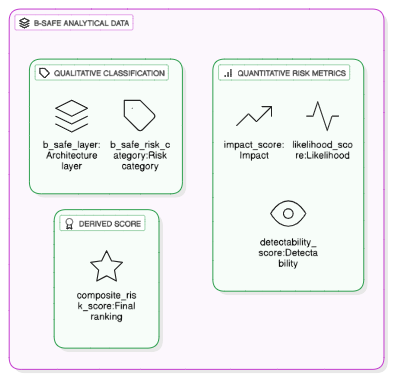
\includegraphics[width=0.3\textwidth]{../figure/methodology/analytical_data.jpg}
        \caption{Analytical data of the dataset.}
        \label{fig:analytical_data}
    \end{figure}
    \item \textbf{b\_safe\_layer}: Assigned B-SAFE architectural layer (NET, CON, SC, PRO, AUX)
    \item \textbf{b\_safe\_risk\_category}: Specific risk category identifier within the B-SAFE framework (e.g., SC-1, PRO-2)
    \item \textbf{impact\_score}: Assigned Impact (I) score on a 1-5 scale, as defined in Section IV.D
    \item \textbf{likelihood\_score}: Assigned Likelihood (L) score on a 1-5 scale, as defined in Section IV.D
    \item \textbf{detectability\_score}: Assigned Detectability (D) score on a 1-5 scale, as defined in Section IV.D
    \item \textbf{composite\_risk\_score}: Calculated priority ranking based on our formula
\end{itemize}

The dataset includes complete risk scoring for all 649 incidents, with 100\% coverage for impact, likelihood, and detectability scores, enabling comprehensive statistical analysis and validation of our risk quantification approach.

\begin{figure}[H]
\centering
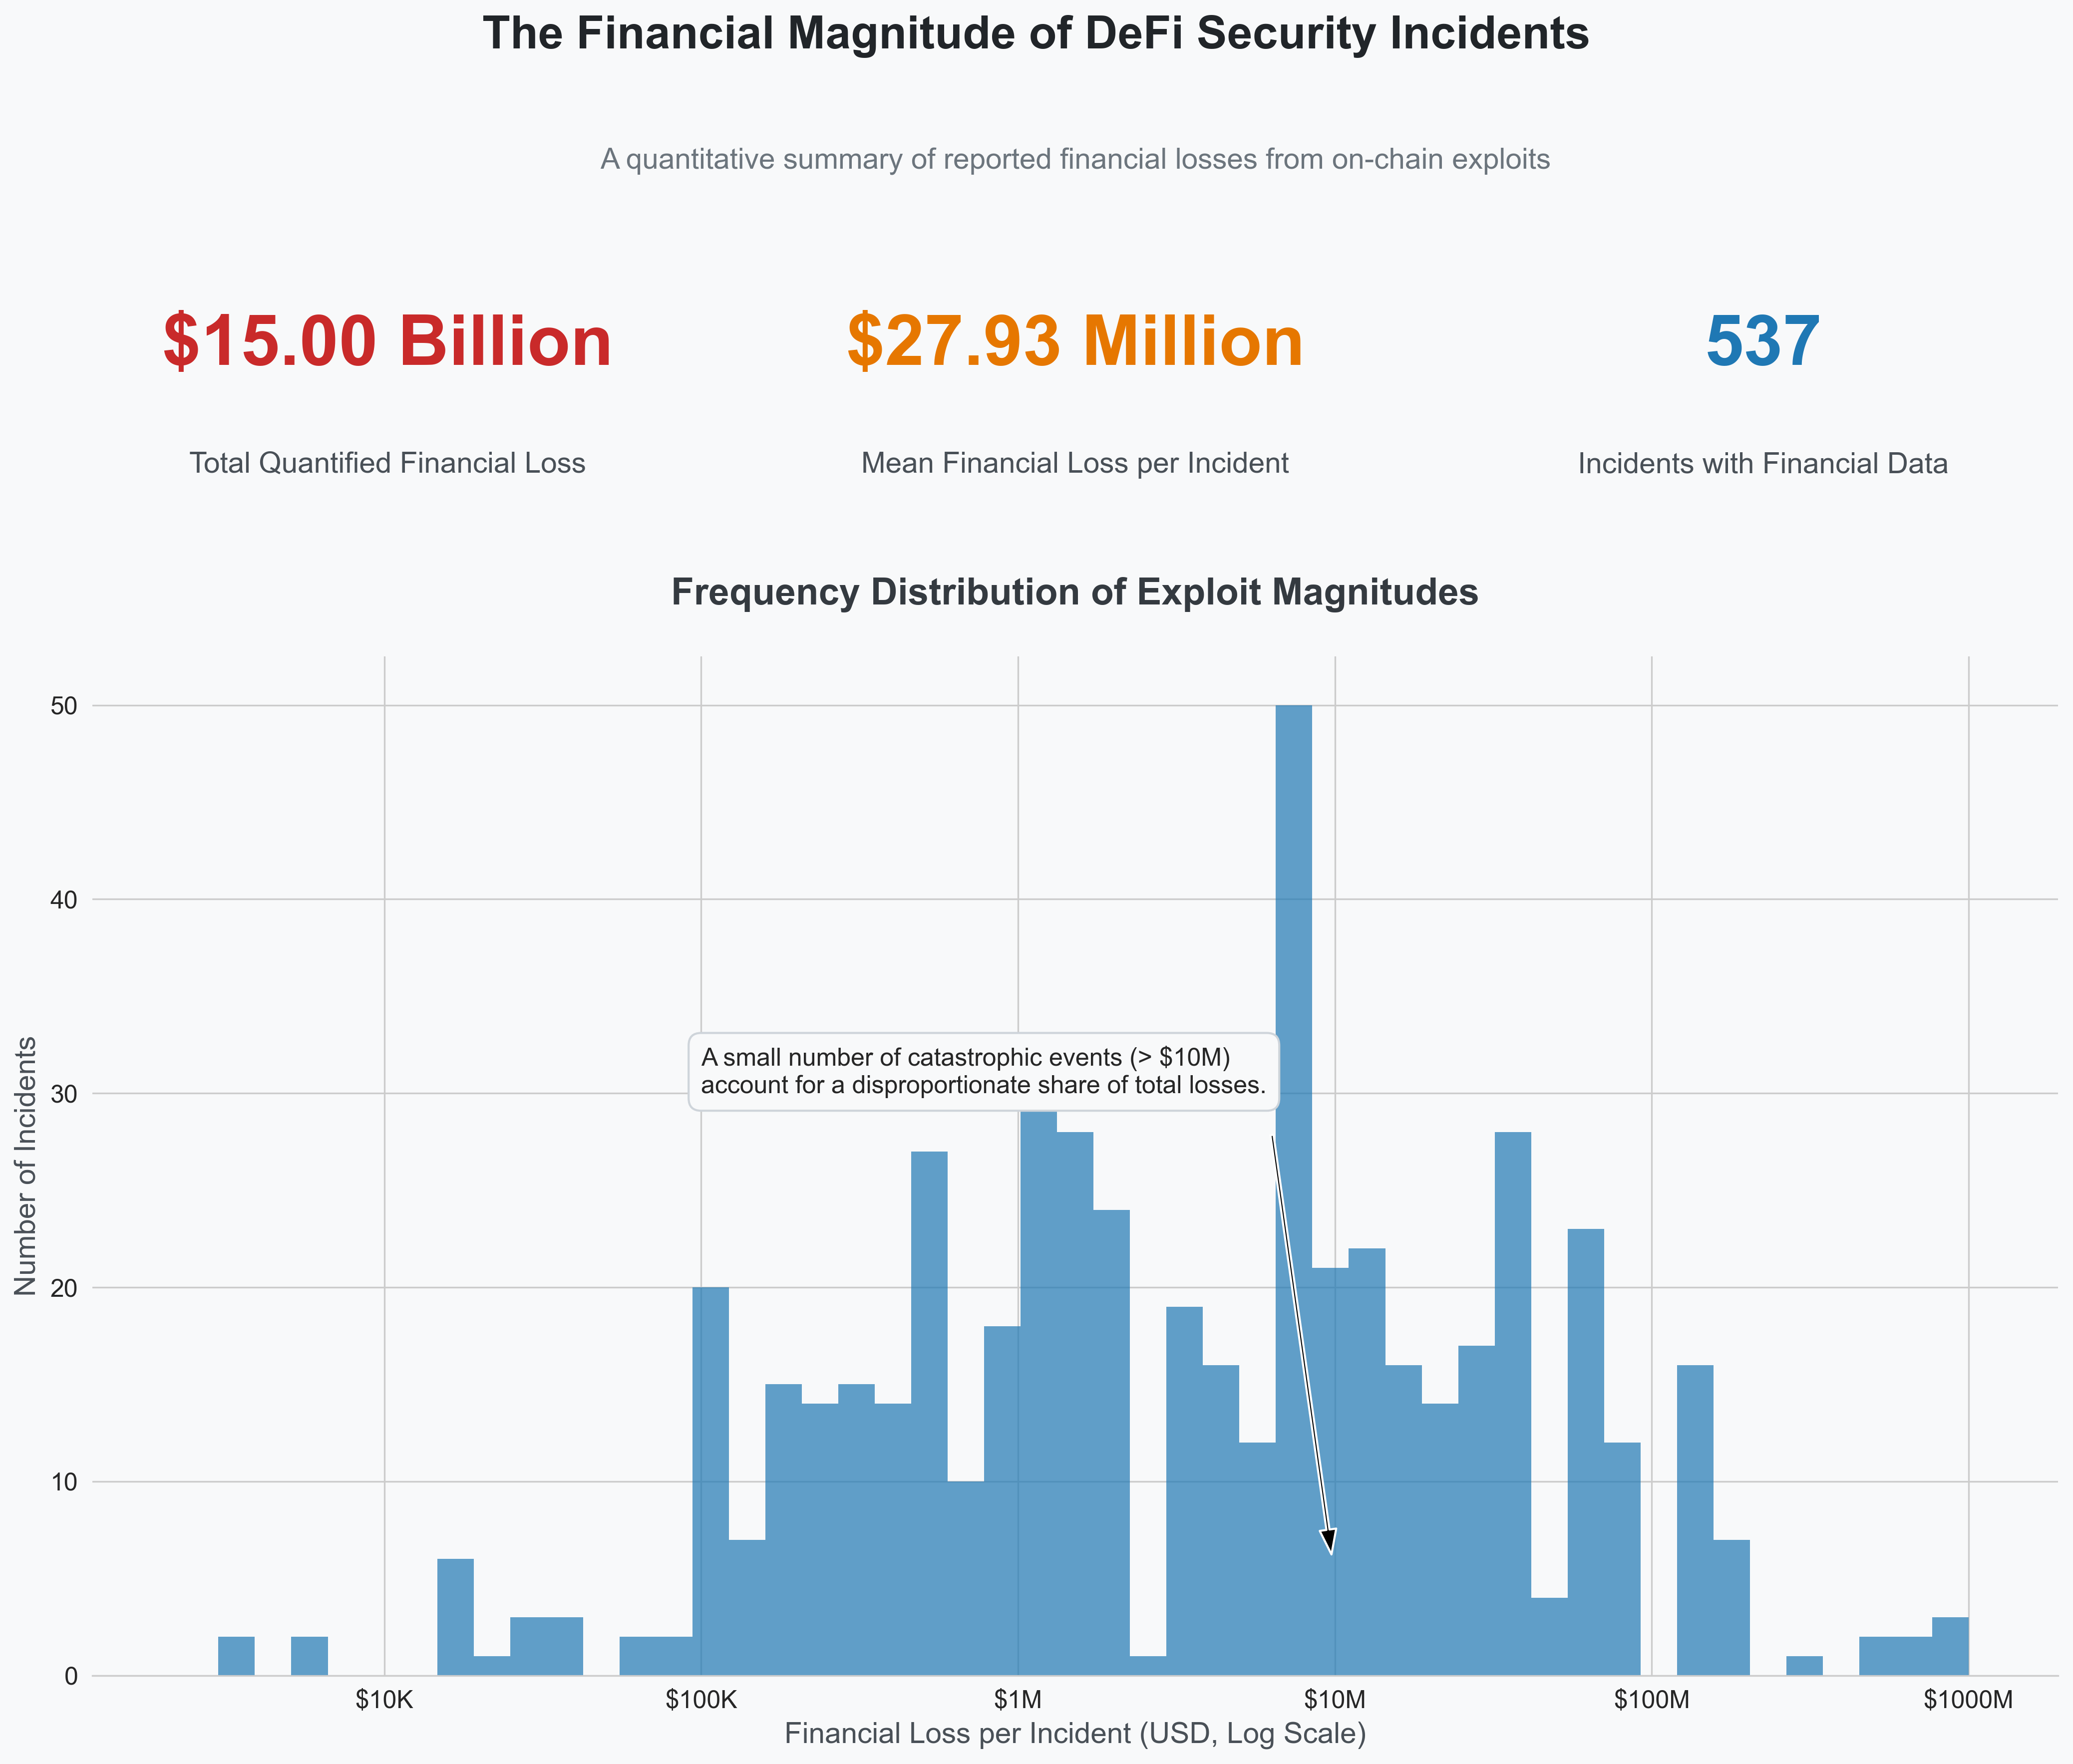
\includegraphics[width=0.5\textwidth]{../figure/methodology/fig4.png}
\caption{Financial Magnitude of DeFi Security Incidents}
\label{fig:data_pipeline}
\end{figure}
